%%%%%%%%%%%%%%%%%%%%%%%%%%%%%%%%%%%%%%%%%
% Journal Article
% LaTeX Template
% Version 1.3 (9/9/13)
%
% This template has been downloaded from:
% http://www.LaTeXTemplates.com
%
% Original author:
% Frits Wenneker (http://www.howtotex.com)
%
% License:
% CC BY-NC-SA 3.0 (http://creativecommons.org/licenses/by-nc-sa/3.0/)
%
%%%%%%%%%%%%%%%%%%%%%%%%%%%%%%%%%%%%%%%%%

%----------------------------------------------------------------------------------------
% PACKAGES AND OTHER DOCUMENT CONFIGURATIONS
%----------------------------------------------------------------------------------------

\documentclass[oneside, 11pt, a4paper]{article}
\usepackage{polski}
\usepackage[utf8]{inputenc} 
\usepackage{cite}

\usepackage{graphicx}

\usepackage{lipsum} % Package to generate dummy text throughout this template

\usepackage[sc]{mathpazo} % Use the Palatino font
\usepackage[T1]{fontenc} % Use 8-bit encoding that has 256 glyphs
\linespread{1.05} % Line spacing - Palatino needs more space between lines
\usepackage{microtype} % Slightly tweak font spacing for aesthetics

%\usepackage[hmarginratio=1:1,top=32mm,columnsep=20pt]{geometry} % Document margins
\usepackage[top=3cm, bottom=3cm, left=2.5cm, right=2.5cm, columnsep=8mm]{geometry}

\usepackage{multicol} % Used for the two-column layout of the document
\usepackage[hang, small,labelfont=bf,up,textfont=it,up]{caption} % Custom captions under/above floats in tables or figures
\usepackage{booktabs} % Horizontal rules in tables
\usepackage{float} % Required for tables and figures in the multi-column environment - they need to be placed in specific locations with the [H] (e.g. \begin{table}[H])
\usepackage{hyperref} % For hyperlinks in the PDF

%\usepackage{lettrine} % The lettrine is the first enlarged letter at the beginning of the text


\usepackage{paralist} % Used for the compactitem environment which makes bullet points with less space between them

\usepackage{abstract} % Allows abstract customization
\renewcommand{\abstractnamefont}{\normalfont\bfseries} % Set the "Abstract" text to bold
\renewcommand{\abstracttextfont}{\normalfont\itshape} % Set the abstract itself to small italic text

\renewenvironment{abstract}
               {\list{}{}%
                \item[\textbf{Streszczenie.}]\relax}
               {\endlist}



\usepackage{titlesec} % Allows customization of titles
\usepackage[labelsep=period,font=small,format=plain,labelfont=bf,textfont=up]{caption}

% \DeclareCaptionFormat{myformat}{\fontsize{10}{11}\selectfont#1#2#3}
% \captionsetup{format=myformat}

\DeclareUnicodeCharacter{00A0}{ } % solution for "Unicode char \u8:  not set up for use with LaTeX."

%\renewcommand\thesection{\Roman{section}} % Roman numerals for the sections
%\renewcommand\thesubsection{\Roman{subsection}} % Roman numerals for subsections
\titleformat{\section}[runin]{\bfseries\centering}{\thesection.}{3pt}{} % Change the look of the section titles
%\titleformat{\subsection}[]{}{}{}{}[]
\titleformat{\subsection}[runin]{\bfseries}{\thesubsection.}{3pt}{} % Change the look of the section titles
\titlespacing*{\section}{0pt}{6pt}{3pt}[0pt]
\titlespacing*{\subsection}{0pt}{3pt}{3pt}[0pt]

\usepackage{fancyhdr} % Headers and footers
\pagestyle{fancy} % All pages have headers and footers
\fancyhead{} % Blank out the default header
\fancyfoot{} % Blank out the default footer
\renewcommand{\headrulewidth}{0pt}

%\fancyhead{} % Custom header text
\fancyfoot[RO,LE]{\begin{center}\thepage\end{center}} % Custom footer text

\renewcommand{\abstractname}{Streszczenie.}    % clear the title
\renewcommand{\absnamepos}{empty} % originally center
\setlength{\parindent}{0.4cm}

 \setlength{\parskip}{0mm}

%----------------------------------------------------------------------------------------
% TITLE SECTION
%----------------------------------------------------------------------------------------

\title{\vspace{15mm}\fontsize{14pt}{10pt}\selectfont\textbf{Problematyka rozproszonych systemów - przypadek \emph{Apache Cassandra}}} % Article title

\author{
{\fontsize{12pt}{1.2em}\selectfont Marek Lewandowski} \\
{\fontsize{11pt}{1.2em}\selectfont Wydział Elektroniki i Technik Informacyjnych, Politechnika Warszawska} \\
{\fontsize{11pt}{1.2em}\selectfont \href{mailto:marek.m.lewandowski@gmail.com}{marek.m.lewandowski@gmail.com}} 
\date{}
}


%----------------------------------------------------------------------------------------

\begin{document}

\maketitle % Insert title

\thispagestyle{fancy} % All pages have headers and footers

%----------------------------------------------------------------------------------------
% ABSTRACT
%----------------------------------------------------------------------------------------



%----------------------------------------------------------------------------------------
% ARTICLE CONTENTS
%----------------------------------------------------------------------------------------

\begin{multicols}{2} % Two-column layout throughout the main article text

%\begin{abstract}
\section*{Streszczenie.}

\textit{
Artykuł omawia nierelacyjne bazy danych i twierdzenia z nimi związane takie jak \emph{CAP, BASE}. W szczególności omawia cechy szczególne i budowę bazy \emph{Apache Cassandra}. \emph{Apache Cassandra} jest kanoniczną nierelacyjną bazą danych, której zrozumienie znacząco ułatwia zrozumienie większości pozostałych nierelacyjnych baz danych.
}

\section{Motywacja.}
Nierelacyjne bazy danych powstały, w celu rozwiązania nowego rodzaju problemów, którym nie były w stanie sprostać tradycyjne bazy danych. Problemy to bardzo duża, szybko przyrastająca ilość danych oraz potrzeba obsługi równie dużego obciążenia systemu.

Ilość danych, wyrażana może być, aż peta bajtach ($1PB=1000 TB$), co może sprawiać problemy jeśli chcielibyśmy obsłużyć taką ilość danych jednym komputerem. W związku z tym poruszamy się po dziedzinie klastrów serwerów, a nie pojedynczych maszyn. Pojedyncza maszyna to również pojedynczy punkt awarii. Takie i inne problemy adresowane są przez nierelacyjne bazy danych.

Często podczas omawiania nierelacyjnych baz danych przytacza się przypadek firmy \emph{Amazon}. \emph{Amazon} oświadczył, że wzrost czasu odpowiedzi w ich serwisie o 0.1 sekundy powoduje spadek sprzedaży o 1\%. Wysoka wydajność i niski czas dostępu są możliwe dzięki nierelacyjnym bazom danych oraz innym pobocznym technikom. Warto zatem pamiętać o biznesowej wartości tych rozwiązań, wiedzieć jak działają i jakim prawom podlegają.

\section{Spójność i dostępność}
W klasycznych bazach danych, często słyszymy o tym, że baza jest spójna. Taka spójność oznacza, że wszystkie mechanizmy w bazie takie jak więzy integralności, klucze obce, ograniczenia na kolumny są spełnione. Chcę przedstawić inną definicję spójności.

Spójność oznacza jedną wersję danych, a więc wszystkie takie same dane, są zawsze w identycznej wersji. Dostępność rozumiana jest jako zdolność systemu do obsługi żądania zapisu/odczytu danych i zwrócenia odpowiedzi. 

\emph{ACID} charakteryzuje klasyczne bazy danych, które posiadają bardzo wysoką spójność. \emph{BASE} to akronim, który należy omówić. 

\begin{compactitem}
  \item większość danych dostępna przez cały czas (ang. Basically Available)
  \item dane wystarczająco świeże (ang. Soft state)
  \item osiągnięcie spójności odsunięte w czasie, ale osiągalne (ang. Eventually consistent)
\end{compactitem}

\emph{ACID} i \emph{BASE} reprezentują dwa podejścia projektowe po przeciwnych końcach spektrum spójność\dywiz dostępność. Naturalnie \emph{ACID} znajduje się po stronie spójności i reprezentuje klasyczne podejście do baz danych. \emph{BASE} znajduje się po przeciwnej stronie spektrum i reprezentuje systemy z dużą dostępnością. Dzięki tym modelom wybór pomiędzy dostępnością, a spójnością jest jawny.


\section{Twierdzenie CAP.}
Brewer opublikował w 1999 roku \cite{Fox99harvest} twierdzenie przedstawiające wybór dwóch z trzech cech w rozproszonych bazach danych. Dwie cechy już znamy. Należy wytłumaczyć czym jest odporność na partycje. 

Partycja w rozprosznym systemie występuje, wtedy gdy część węzłów w klastrze nie ma łączności z co najmniej jednym węzłem, inaczej mówiąc klaster jest podzielony na dwie części, które nie mogą się ze sobą komunikować. Taka sytuacja może wystąpić w co najmniej dwóch przypadkach. Część maszyn może ulec awarii i tym samym zniknie z klastra na długi czas, a więc będzie niedostępna z punktu widzenia pozostałych maszyn. Inną możliwością jest brak łączności spowodowany awarią sieci. Z punktu widzenia maszyn w klastrze obie sytuacje są identyczne i nie da się ich rozróżnić. W obu tych sytuacjach występuje partycja rozdzielająca maszyny na dwie grupy.
 Twierdzenie Brewera mówi, że można mieć jedynie dwie cechy z poniższych:
\begin{compactitem}
  \item spójność,
  \item dostępność,
  \item odporność na partycje.
\end{compactitem}

W przypadku rozproszonych systemów brak odporności na partycje to pojedyczny punkt awarii. Wystarczy sobie wyobrazić, że pojedyncza maszyna ulega awarii, a baza nie jest w stanie dalej funkcjonować. Z tego powodu rozważa się wybór pomiędzy dostępnością, a spójnością. Odporność na partycje powinna być zawsze. Można zatem mówić o binarnym wyborze.

Binarny wybór został zaprezentowany w oryginalnej postaci twierdzenia. Przez ponad dekadę powstało wiele typów systemów, które skupiają się na innych kombinacjach właściwości. 
\subsection{Twierdzenie dzisiaj.} Wokół twierdzenia pojawiło się wiele nieporozumień. Przez lata odkryto sporo niuansów. Właściwości nie są binarne, a bliżej im do wartości ciągłych. Dostępność jest w zakresie procentowym. Istnieje wiele poziomów spójności. Węzły w klastrze mogą nie zgadzać się co do tego czy partycja faktycznie występuje. Autor opublikował 12 lat później artykuł \cite{Brewer:2012ba}, który rozwiewa większość wątpliwości.

Dzisiaj możemy przedstawić twierdzenie w lepszy sposób. Podczas wystąpienia partycji niemożliwa jest idealna spójność i idealna dostępność. Dzięki specjalnej obsłudze systemu podczas partycji, można mieć więcej niż tylko jedną cechę. Wymaga to użycia odpowiednik technik. Jedną z technik jest ograniczenie możliwych operacji, tylko do tych, które nie zniszczą spójności. Przykładem rozprosznego systemu, który stosuje taką technikę jest \emph{Google Docs}, który podczas braku połączenia (partycji), udostępnia tylko część narzędzi tesktowych. 

Jeśli partycja nie występuje system może mieć idealną dostępność i spójność. Dopiero podczas wystąpienia partycji należy dokonać wyboru pomiędzy spójnością, a dostępnością lub mieć specjalny tryb operacji podczas partycji. Nie dokonanie wyboru w krótkim czasie to wybór spójności, ponieważ żądanie nie zostanie obsłużone w odpowiednim czasie, a więc z perspektywy klienta system nie będzie dostępny.

\section{Parametry nierelacyjnych baz danych.}

\subsection{Reguła spójności.}

\section{Apache Cassandra.}

\subsection{Liniowa skalowalność.}

\subsection{Natywny model danych.}

\subsection{Model CQL.}

\subsection{Przypadki użycia.}

\section{Motywacja.}


 \begin{figure}[H]
  \fbox{
    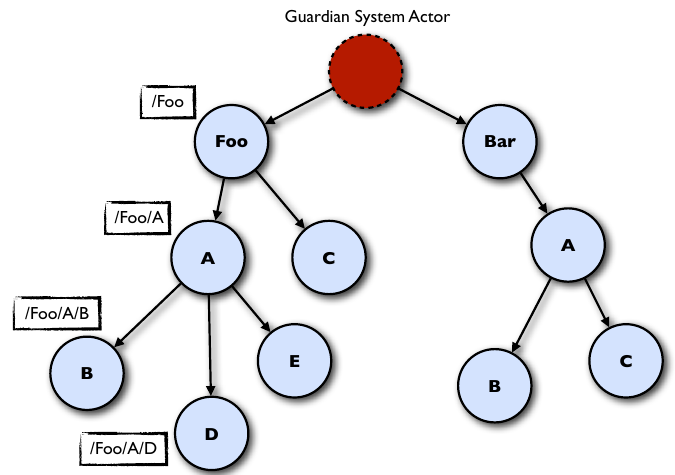
\includegraphics[scale=0.36]{./fig-actor-hierarchy.png}
  }
  \begin{center}
  \caption{A picture of the same gull
           looking the other way!}
  \end{center}
  
\end{figure}



%------------------------------------------------
%
%
%
%\section{Results}
%
%\begin{table}[H]
%\caption{Example table}
%\centering
%\begin{tabular}{llr}
%\toprule
%\multicolumn{2}{c}{Name} \\
%\cmidrule(r){1-2}
%First name & Last Name & Grade \\
%\midrule
%John & Doe & $7.5$ \\
%Richard & Miles & $2$ \\
%\bottomrule
%\end{tabular}
%\end{table}
%
%\lipsum[5] % Dummy text
%
%\begin{equation}
%\label{eq:emc}
%e = mc^2
%\end{equation}
%
%\lipsum[6] % Dummy text

%------------------------------------------------



%----------------------------------------------------------------------------------------
% REFERENCE LIST
%----------------------------------------------------------------------------------------

\bibliography{bibliography}{}
\bibliographystyle{plain}


%----------------------------------------------------------------------------------------

\end{multicols}

\end{document}